\documentclass{article}

\usepackage[utf8]{inputenc}
\usepackage[T1]{fontenc}
\usepackage[spanish, es-tabla]{babel}
\usepackage{csquotes}

\usepackage{geometry}
\geometry{a4paper, margin=1in}
\usepackage{xcolor}
\usepackage{fancyhdr}
\usepackage{titlesec}
\usepackage{enumitem}
\usepackage{parskip} 
\setlength{\parskip}{0.8em}

\usepackage{amsmath, amsfonts, amssymb, amsthm}
\usepackage{bm}
\usepackage{cancel}
\usepackage{matlab-prettifier}

\usepackage{graphicx}
\usepackage{float}
\usepackage{subfig}
\usepackage{bookmark}
\usepackage[most]{tcolorbox}
\usepackage{array, tabularx, longtable}
\newcolumntype{E}{>{$}c<{$}}
\setcounter{MaxMatrixCols}{40}

\usepackage{tikz, pgfplots}
\usepackage[americanvoltages, fulldiodes, siunitx]{circuitikz}
\usetikzlibrary{calc, patterns, quotes, angles}
\pgfplotsset{compat=1.18}

\setlength{\headheight}{16pt} 
\pagestyle{fancy}
\fancyhf{}
\fancyhead[L]{Yaiza M. Martín}
\fancyhead[R]{Informe Prácticas - IAC}
\fancyfoot[C]{\thepage}

\usepackage{hyperref}


\title{Informe Prácticas}
\author{Yaiza María Martín Mesones}
\date{2026}

\begin{document}

\begin{titlepage}
    \begin{center}
        \vspace*{3cm} 
        \Huge \textbf{Informe de Prácticas Externas}\\[0.75cm]
        \Large \textsc{Recalibración de la espectrofotometría de Gaia basándose en CALSPEC mediante Técnicas de Aprendizaje Automático}
                
        \vfill
        \Large \textbf{Autora:}\\[0.2cm]
        \large Yaiza María Martín Mesones \\
        \small \textit{Grado en Matemáticas}
        
        \vfill 
        \Large \textbf{Universidad de La Laguna} \\
        \textit{Facultad de Ciencias} \\
        \textit{Instituto de Astrofísica de Canarias (IAC)} \\
        \vspace{1cm}
        {\Large Junio 2026}
    \end{center}
\end{titlepage}

\newpage
\clearpage
\tableofcontents


\newpage
\begin{figure}[H]
    \centering
    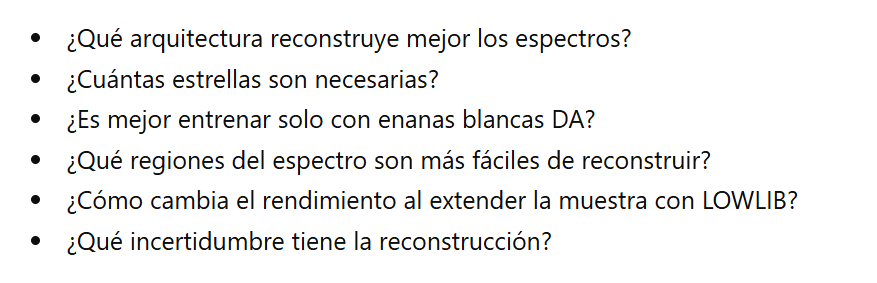
\includegraphics[width=0.5\linewidth]{image.png}
    \caption{Enter Caption}
    \label{fig:placeholder}
\end{figure}

\newpage
\section{Introducción}

La astrofísica moderna depende en gran medida del análisis de grandes volúmenes de datos observacionales y de la interpretación precisa de la información espectral procedente de estrellas y otros objetos celestes. En este contexto, misiones como \textit{Gaia} han revolucionado la forma en que se estudia la estructura y evolución de la Vía Láctea, proporcionando mediciones extremadamente precisas de posiciones, movimientos y propiedades fotométricas de millones de estrellas.

Paralelamente, los espectros estelares de referencia, como los proporcionados por el conjunto CALSPEC, constituyen una base fundamental para la calibración de instrumentos y la interpretación física de las observaciones astronómicas. La relación entre espectros de alta resolución y las observaciones fotométricas en bandas amplias como BP y RP es un problema clave en la conversión entre modelos físicos y datos observacionales.

Es por ello, que se estudiará la relación entre espectros estelares y observaciones simuladas en el sistema fotométrico de Gaia, mediante técnicas de procesamiento de datos y aprendizaje automático. En particular, se exploran métodos computacionales que permiten aproximar dicha relación de forma eficiente y analizar la capacidad de generalización de modelos basados en redes neuronales.

\subsection{Contexto del problema}

La misión Gaia de la Agencia Espacial Europea ha proporcionado un catálogo de observaciones astrométricas y fotométricas de más de mil millones de estrellas. Entre sus productos más relevantes se encuentran las magnitudes en las bandas BP (\textit{Blue Photometer}) y RP (\textit{Red Photometer}), que constituyen una representación de baja resolución del espectro estelar.

Por otro lado, CALSPEC es un conjunto de espectros de calibración de alta precisión que se utiliza como referencia absoluta en fotometría astronómica. Sin embargo, la relación directa entre estos espectros de alta resolución y las observaciones de Gaia no es trivial, ya que implica la convolución con la respuesta instrumental del satélite, y efectos tanto de muestreo como de ruido.

Este problema puede abordarse desde un punto de vista físico o estadístico. En este trabajo se adopta un enfoque computacional, combinando simulación de observaciones con técnicas de aprendizaje automático para modelar la relación entre ambos espacios de datos. 

\subsection{Objetivos del trabajo}
El objetivo principal de este trabajo es analizar la relación entre espectros estelares de referencia y observaciones fotométricas simuladas del sistema Gaia BP/RP mediante técnicas computacionales.

Mas concretamente, se busca:

\begin{itemize}
    \item Construir un conjunto de datos a partir de espectros CALSPEC y observaciones de Gaia.
    \item Simular observaciones fotométricas BP/RP a partir de espectros de alta resolución.
    \item Implementar métodos de aprendizaje automático para modelar la relación entre espectros y observaciones.
    \item Evaluar el rendimiento de distintos modelos en términos de error de predicción y capacidad de generalización.
    \item Analizar el comportamiento del modelo en distintos subconjuntos físicos de estrellas, como enanas blancas.
    \item Explorar la posible ampliación del conjunto de datos mediante catálogos adicionales como LOWLIB.
\end{itemize}

\subsection{Estructura del informe}
El trabajo se estructura de la siguiente manera:

En la Sección 2 se presenta una revisión bibliográfica sobre espectros estelares, el sistema fotométrico de Gaia y el uso de técnicas de aprendizaje automático en astrofísica. 

En la Sección 3 se describe el entorno computacional utilizado, incluyendo las herramientas y librerías empleadas para el análisis de datos. 

En la Sección 4 se detalla el proceso de obtención, cruce y preprocesado de los datos procedentes de CALSPEC y Gaia. 

En la Sección 5 se expone el procedimiento de simulación de observaciones BP/RP a partir de espectros estelares.

En la Sección 6 se presentan los modelos de aprendizaje automático implementados y su metodología de entrenamiento.

En la Sección 7 se analizan los resultados obtenidos y se evalúa el rendimiento de los modelos.

En la Sección 8 se discute la posible ampliación del conjunto de datos mediante LOWLIB.

Finalmente, en la Sección 9 se recogen las conclusiones del trabajo y posibles líneas futuras de investigación.


\newpage
\section{Revisión bibliográfica}

\subsection{Espectros estelares y calibración fotométrica}

Los espectros estelares constituyen una herramienta fundamental en astrofísica para inferir propiedades físicas como la temperatura efectiva, la metalicidad o la gravedad superficial. La distribución espectral de energía de una estrella contiene información detallada sobre los procesos físicos que tienen lugar en su atmósfera.

Sin embargo, en muchos contextos observacionales no se dispone de espectros de alta resolución, sino de medidas fotométricas integradas en bandas anchas. Estas observaciones pueden interpretarse como integrales ponderadas del espectro original, lo que implica una pérdida significativa de información espectral.

Por ello, la calibración fotométrica requiere el uso de espectros de referencia bien caracterizados, que permitan establecer relaciones entre magnitudes observadas y flujos físicos absolutos.

\subsection{CALSPEC: características y uso en astrofísica}

El conjunto CALSPEC constituye el estándar de referencia en calibración espectrofotométrica absoluta. Desarrollado por el Space Telescope Science Institute, proporciona espectros de alta precisión calibrados en flujo absoluto para un conjunto de estrellas estándar \cite{bohlin2014}.

Estos espectros han sido utilizados para la calibración de instrumentos en múltiples misiones espaciales, incluyendo el telescopio espacial Hubble. Su alta precisión y cobertura espectral los convierten en una herramienta fundamental para validar modelos instrumentales y generar simulaciones de observaciones.

\vspace{0.25cm} En el contexto de este trabajo, CALSPEC se emplea como base para construir un conjunto de datos en el que se dispone del espectro completo, lo que permite estudiar su relación con observaciones fotométricas de menor resolución.

\subsection{Gaia BP/RP: instrumentación y datos}

La misión Gaia de la Agencia Espacial Europea ha supuesto un avance sin precedentes en el estudio de la Vía Láctea, proporcionando datos astrométricos y fotométricos de más de mil millones de estrellas \cite{gaia2016}.

Entre sus instrumentos, los fotómetros BP (Blue Photometer) y RP (Red Photometer) proporcionan una representación de baja resolución del espectro estelar mediante prismas dispersivos. Los datos correspondientes han sido publicados en diferentes versiones del catálogo, siendo Gaia Data Release 3 una de las más completas hasta la fecha \cite{gaia2022}.

Estas observaciones no corresponden a espectros continuos tradicionales, sino a distribuciones de flujo muestreadas en un número limitado de puntos, lo que introduce dificultades adicionales en su interpretación y modelado.

\subsection{Relación entre espectros y observaciones fotométricas}

La relación entre un espectro estelar y sus observaciones fotométricas puede describirse mediante una transformación integral que incorpora la respuesta instrumental del sistema \cite{bessell2012}.

Este proceso implica una reducción de dimensionalidad, ya que la información espectral original se proyecta en un conjunto limitado de observables. Como consecuencia, la transformación no es trivialmente invertible, lo que dificulta la reconstrucción del espectro a partir de datos fotométricos.

Diversos enfoques han sido propuestos para abordar este problema, incluyendo modelos físicos basados en atmósferas estelares y métodos estadísticos orientados a la aproximación de la transformación.

\subsection{Machine Learning en astrofísica}

El aprendizaje automático ha emergido como una herramienta clave en el análisis de grandes volúmenes de datos astronómicos \cite{baron2019}. Su capacidad para modelar relaciones no lineales complejas lo hace especialmente adecuado para problemas en los que no existe una formulación analítica sencilla.

En particular, las redes neuronales han sido aplicadas con éxito en la estimación de parámetros estelares y en la modelización de espectros a partir de datos observacionales \cite{ting2019}. Estos métodos permiten aproximar funciones complejas sin necesidad de un modelo físico explícito.

En este trabajo se adopta este enfoque para modelar la relación entre espectros de alta resolución (CALSPEC) y observaciones fotométricas en el sistema Gaia BP/RP, evaluando la capacidad de distintos modelos para capturar dicha transformación.




\newpage
\section{Entorno computacional y herramientas}

\subsection{Lenguaje de programación y librerías}

El desarrollo de este trabajo se ha realizado principalmente en el lenguaje de programación Python, debido a su amplia adopción en el ámbito de la ciencia de datos y la astrofísica computacional. Python proporciona un ecosistema de librerías científicas que permiten la manipulación eficiente de datos, el cálculo numérico y la implementación de modelos de aprendizaje automático.

Entre las principales librerías utilizadas se encuentran:

\begin{itemize}
    \item \textbf{NumPy}: para el cálculo numérico eficiente y la manipulación de arrays multidimensionales.
    \item \textbf{SciPy}: para métodos numéricos avanzados, interpolación y procesamiento científico.
    \item \textbf{Pandas}: para la gestión y análisis de datos tabulares.
    \item \textbf{Matplotlib}: para la visualización de datos y representación gráfica de resultados.
    \item \textbf{Astropy}: para el manejo de datos astronómicos y formatos estándar en astrofísica.
    \item \textbf{Scikit-learn}: para la implementación de modelos de aprendizaje automático clásicos.
    \item \textbf{PyTorch}: para el desarrollo y entrenamiento de redes neuronales.
\end{itemize}

\subsection{Estructura del proyecto}

Con el objetivo de garantizar la reproducibilidad y la organización del trabajo, el proyecto se ha estructurado en diferentes directorios funcionales:

\begin{itemize}
    \item \texttt{data/}: contiene los conjuntos de datos originales y procesados, incluyendo espectros CALSPEC y datos de Gaia.
    \item \texttt{src/}: código fuente principal del proyecto, incluyendo funciones de preprocesado, simulación y modelos.
    \item \texttt{results/}: resultados obtenidos, figuras generadas y métricas de evaluación.
    \item \texttt{docs/}: documentación adicional y notas técnicas.
\end{itemize}

Esta estructura permite separar claramente los datos, el código y los resultados, facilitando la reproducibilidad del estudio.

\subsection{Gestión de datos y reproducibilidad}

La gestión adecuada de los datos es un aspecto fundamental en cualquier proyecto científico. En este trabajo, los datos procedentes de CALSPEC y Gaia han sido almacenados y procesados siguiendo criterios de reproducibilidad y trazabilidad.

Se ha intentado garantizar que todos los pasos del análisis puedan ser reproducidos a partir del código fuente, evitando procesos manuales no documentados. Para ello, se han utilizado scripts automatizados que permiten desde la descarga de datos hasta la generación de resultados finales. Asimismo, se ha prestado especial atención a la consistencia de las versiones de las librerías utilizadas, con el fin de asegurar que los resultados obtenidos sean reproducibles en diferentes entornos computacionales. Finalmente, se ha considerado la posibilidad de alojar el código en un repositorio de control de versiones, lo que facilita el seguimiento de cambios y la colaboración en proyectos de investigación futuros.


\newpage
\section{Obtención y preparación de datos}

\subsection{Descarga de espectros CALSPEC}

El conjunto de datos CALSPEC se ha obtenido a partir de su repositorio oficial, que proporciona espectros estelares de alta precisión calibrados en flujo absoluto. Estos espectros constituyen una referencia estándar en astrofísica observacional.

Una vez descargados, los datos han sido organizados en un formato homogéneo para su posterior procesamiento. Debido a la diversidad de resoluciones espectrales y rangos de longitud de onda, ha sido necesario realizar un tratamiento previo para asegurar la comparabilidad entre diferentes muestras.

En esta fase se han eliminado entradas incompletas o no utilizables, y se ha verificado la consistencia de las unidades físicas asociadas a los espectros.

\subsection{Obtención de datos Gaia BP/RP}
Los datos fotométricos correspondientes a las bandas BP (Blue Photometer) y RP (Red Photometer) de la misión Gaia han sido obtenidos a partir de los catálogos públicos disponibles.

Estos datos proporcionan una representación de baja resolución del espectro estelar, resultado de la convolución del espectro original con la respuesta instrumental del satélite. Debido a la gran cantidad de observaciones disponibles, se ha realizado una selección de subconjuntos relevantes para este estudio.

\subsection{Cruce de catálogos (cross-match)}

Para poder relacionar los espectros CALSPEC con las observaciones de Gaia, se ha llevado a cabo un proceso de cruce de catálogos (cross-match).
Este procedimiento consiste en identificar objetos astronómicos comunes entre ambas bases de datos mediante criterios de coincidencia en posición y otros parámetros astrofísicos relevantes. El resultado de dicho proceso es un conjunto de estrellas para las cuales se dispone tanto de espectros de alta resolución como de observaciones fotométricas en BP/RP, lo que permite establecer relaciones entre ambos espacios de datos.

\subsection{Preprocesado y limpieza de datos}

Una vez obtenidos los conjuntos de datos, se ha procedido a su preprocesado con el objetivo de mejorar su calidad y adecuación para el análisis computacional.
Entre las principales operaciones realizadas se incluyen:

\begin{itemize}
    \item Eliminación de valores atípicos o inconsistentes.
    \item Normalización de los espectros para asegurar escalas comparables.
    \item Interpolación de datos espectrales para obtener una rejilla común de longitudes de onda.
    \item Sincronización de los conjuntos CALSPEC y Gaia en un espacio de características común.
\end{itemize}

Este proceso es fundamental para garantizar que los modelos posteriores de aprendizaje automático operen sobre datos coherentes y homogéneos.

\subsection{Normalización e interpolación de espectros}

Dado que los espectros CALSPEC presentan distintas resoluciones y muestreos en longitud de onda, ha sido necesario aplicar técnicas de interpolación para representar todos los espectros sobre una misma rejilla espectral.

Además, se ha realizado una normalización de los espectros con el objetivo de eliminar efectos de escala y facilitar el aprendizaje por parte de los modelos computacionales. Esta normalización permite centrar el análisis en la forma del espectro más que en su amplitud absoluta.

Este paso resulta esencial para la posterior aplicación de técnicas de simulación y aprendizaje automático, ya que reduce la variabilidad no relevante de los datos y mejora la estabilidad numérica de los algoritmos.


\newpage
\newpage
\section{Procesamiento de espectros y degradación de resolución}

\subsection{El problema de la resolución instrumental}

Los datos espectrofotométricos de Gaia (bandas BP/RP) presentan una resolución significativamente menor y un aspecto más suavizado que los espectros de alta precisión proporcionados por el Telescopio Espacial Hubble en el catálogo CALSPEC. Esta discrepancia se debe a las diferencias en el diseño óptico, la dispersión de los prismas y la función de respuesta instrumental de cada satélite.

Para poder comparar ambas bases de datos y entrenar un modelo de aprendizaje automático, no es posible utilizar los espectros originales de CALSPEC de forma directa, pues es necesario transformar la "verdad absoluta" del Hubble para que emule las condiciones de observación e instrumentación propias de Gaia. De este modo, se consigue eliminar el exceso de resolución, pero conservando la precisión de flujo característica de CALSPEC.

\subsection{Degradación espectral mediante convolución}

El primer paso del procesamiento consiste en reducir la resolución de los espectros de CALSPEC. Este proceso de degradación se modela matemáticamente mediante la convolución del espectro de alta resolución original, $F_{\text{HST}}(\lambda)$, con una función de dispersión instrumental (LSF, \textit{Line Spread Function}), que a menudo se aproxima mediante un núcleo gaussiano o a través de las matrices de dispersión oficiales proporcionadas por el consorcio de Gaia:

\begin{equation}
F_{\text{degradado}}(\lambda) = \int F_{\text{HST}}(\lambda') \, K(\lambda, \lambda') \, d\lambda',
\end{equation}

donde $K(\lambda, \lambda')$ representa el núcleo de la transformación que simula el suavizado instrumental de Gaia. El resultado es un espectro sintético que representa cómo vería el Hubble esa misma estrella si tuviera las limitaciones de resolución del instrumento BP/RP de Gaia, pero libre de los errores sistemáticos y de calibración que queremos corregir.

\subsection{Alineación de rejilla e interpolación}

Una vez degradados los espectros de CALSPEC, el siguiente reto radica en que los flujos de ambas bases de datos no están evaluados en los mismos puntos de longitud de onda. Los espectros reales de Gaia se distribuyen en un número fijo de píxeles o coeficientes internos.

Para asegurar la consistencia dimensional en los vectores de entrada del modelo de regresión, se implementa un proceso de remuestreo e interpolación numérica (utilizando splines cúbicos o interpolación lineal optimizada mediante \texttt{SciPy}). Ambos espectros —el de Gaia con errores sistemáticos y el de CALSPEC degradado y limpio— se proyectan sobre una rejilla común y homogénea de longitudes de onda:

\begin{equation}
\mathbf{\Lambda} = [\lambda_1, \lambda_2, \dots, \lambda_N]
\end{equation}

\subsection{Análisis de residuos y preparación del dataset}

Con los espectros de Gaia y CALSPEC evaluados en la misma rejilla dimensional, se procede a calcular el vector de residuos inicial para la muestra de estrellas comunes (principalmente enanas blancas):

\begin{equation}
\mathbf{R}(\lambda) = \mathbf{F}_{\text{Gaia}}(\lambda) - \mathbf{F}_{\text{CALSPEC\_degradado}}(\lambda)
\end{equation}

El análisis estadístico de estos residuos ($\mathbf{R}$) permite caracterizar de forma preliminar la naturaleza de los errores de Gaia:
\begin{itemize}
    \item \textbf{Errores sistemáticos:} Desviaciones consistentes o sesgos en determinadas longitudes de onda provocados por imperfecciones en el calibrado instrumental del satélite. Estos sesgos no lineales constituyen el objetivo primordial que la red neuronal deberá aprender a corregir.
    \item \textbf{Errores aleatorios:} Dispersión y ruido estadístico propio de las observaciones, que delimitarán el margen de error mínimo factible en nuestra recalibración.
\end{itemize}

El conjunto de pares ordenados $\{\mathbf{F}_{\text{Gaia}}, \mathbf{F}_{\text{CALSPEC\_degradado}}\}$ constituye el dataset definitivo que se introducirá en los algoritmos de aprendizaje automático para llevar a cabo la corrección generalizada.



\newpage
\newpage
\section{Modelos de aprendizaje automático}

\subsection{Definición del problema de regresión y dirección del modelo}

El objetivo central de esta fase es modelar y corregir de forma automatizada los errores sistemáticos y aleatorios presentes en las observaciones fotométricas de \textit{Gaia} DR3 (bandas BP/RP), utilizando como referencia absoluta los espectros de alta precisión del catálogo CALSPEC obtenidos por el Telescopio Espacial Hubble.

Este fenómeno se formula matemáticamente como un problema de regresión supervisada multivariante (o aprendizaje de operadores funcionales). El conjunto de características de entrada ($\mathcal{X}$) está constituido por las representaciones de los espectros observados o vectores de coeficientes procedentes de Gaia, los cuales arrastran sesgos instrumentales y efectos de modelado físico. Por su parte, el conjunto de salida u objetivo ($\mathcal{Y}$) corresponde a los espectros de CALSPEC previamente degradados a la resolución instrumental de Gaia, actuando como la "verdad absoluta" (\textit{ground truth}) exenta de errores sistemáticos.

El modelo de aprendizaje automático busca aproximar un operador o función de mapeo $f$ tal que:

\begin{equation}
f: \mathcal{X}_{\text{Gaia}} \rightarrow \mathcal{Y}_{\text{CALSPEC\_degradado}}
\end{equation}

Al entrenar el algoritmo sobre este espacio, la red neuronal aprende de forma implícita las funciones inversas de corrección de errores de los instrumentos de Gaia, permitiendo su posterior aplicación generalizada a todo el catálogo galáctico.

\subsection{Modelos clásicos de referencia (baseline)}

Como paso inicial en el diseño estadístico, se implementan modelos de aprendizaje automático clásicos utilizando la librería \texttt{Scikit-learn}. Estos modelos sirven como línea base cuantitativa para evaluar si la complejidad de las arquitecturas de aprendizaje profundo está matemáticamente justificada.

Entre los modelos de regresión multivariante considerados se incluyen:
\begin{itemize}
    \item \textbf{Regresión Lineal Multivariable / Regresión Ridge:} Para evaluar si las correcciones sistemáticas guardan una relación lineal o si existe multicolinealidad en las bandas de longitud de onda.
    \item \textbf{Random Forest Regressor:} Un modelo no paramétrico basado en ensamblados de árboles de decisión, altamente robusto frente a la dimensionalidad y capaz de capturar interacciones no lineales de primer orden sin asumir distribuciones previas.
    \item \textbf{Support Vector Regression (SVR):} Configurado con núcleos (kernels) no lineales como el Gaussiano (RBF), el cual proyecta las características de Gaia a un espacio de Hilbert de dimensiones superiores para encontrar hiperplanos de separación óptimos que minimicen el error de calibración.
\end{itemize}

\subsection{Redes neuronales artificiales}

\begin{sloppypar}
Posteriormente, se implementan arquitecturas de redes neuronales artificiales profundas utilizando \texttt{PyTorch}. Debido a la naturaleza continua y correlacionada de los flujos espectrales, las redes neuronales son idóneas para aproximar los mapas de corrección altamente no lineales del satélite.
\end{sloppypar}

Formalmente, definimos $x \in \mathbb{R}^{N}$ como el vector que representa el espectro de entrada de Gaia, $y \in \mathbb{R}^{N}$ el correspondiente espectro de referencia calibrado de CALSPEC, siendo $\hat{y} = f_{\theta}(x)$ la predicción continua producida por una red neuronal parametrizada por sus pesos y sesgos $\theta$. Aquí, $N$ representa el número de muestras o canales de la rejilla homogénea de longitud de onda común, $y_i$ es el flujo de referencia a la longitud de onda $\lambda_i$, $\hat{y}_i$ el flujo predicho por el modelo, y $\Delta\lambda_i$ representa el espaciado o paso discreto entre longitudes de onda consecutivas.

Dada la escala relativamente reducida de la muestra inicial (decenas de objetos de CALSPEC comunes), se opta por un Perceptrón Multicapa (MLP) con regularización estricta mediante capas de \textit{Dropout} y penalizaciones $L_2$ para mitigar de forma rigurosa el riesgo de sobreajuste (\textit{overfitting}).

\subsection{Funciones de pérdida estándar y entrenamiento}

El ajuste de los parámetros libres $\theta$ de la red se guía por la minimización de un funcional de coste. En este trabajo se evalúan y comparan tres funciones de pérdida tradicionales en problemas de regresión:

\subsubsection{Mean Squared Error (MSE)}
El Error Cuadrático Medio se define como:
\begin{equation}
L_{\mathrm{MSE}} = \frac{1}{N} \sum_{i=1}^{N} \left(y_i-\hat{y}_i\right)^2
\end{equation}
Este objetivo penaliza fuertemente las desviaciones grandes debido a su naturaleza cuadrática, obligando a la red a corregir sesgos macroscópicos, aunque presenta una alta sensibilidad a ruidos atípicos puntuales.

\subsubsection{Mean Absolute Error (MAE)}
El Error Absoluto Medio se define matemáticamente como:
\begin{equation}
L_{\mathrm{MAE}} = \frac{1}{N} \sum_{i=1}^{N} |y_i-\hat{y}_i|
\end{equation}
A diferencia de MSE, MAE proporciona una penalización puramente lineal, otorgando una gran estabilidad e inmunidad estadística frente a valores atípicos (\textit{outliers}) o artefactos de reducción de datos presentes en los canales extremos de los fotómetros de Gaia.

\subsubsection{Huber Loss}
Como solución híbrida de compromiso, la pérdida de Huber combina las propiedades analíticas del comportamiento cuadrático para errores pequeños y el comportamiento lineal para errores grandes. Definiendo el residuo como $e_i = y_i - \hat{y}_i$, se establece que:
\begin{equation}
L_{\mathrm{Huber}} = \frac{1}{N} \sum_{i=1}^{N} \ell_{\delta}(e_i)
\end{equation}
donde el término de penalización umbralizado viene dado por:
\begin{equation}
\ell_{\delta}(e)=
\begin{cases}
\dfrac{1}{2}e^{2}, & |e|<\delta, \\[0.3cm]
\delta\left(|e|-\dfrac{\delta}{2}\right), & |e|\geq\delta,
\end{cases}
\end{equation}
y donde $\delta > 0$ es un hiperparámetro crítico de sintonización que controla la transición exacta entre ambos regímenes de optimización.

\subsection{Función de pérdida informada por la física (Physics-Informed Loss)}

Dado que los espectros estelares obedecen a leyes físicas subyacentes de transferencia radiativa y conservación de la energía en las atmósferas estelares, el modelo puede mejorarse drásticamente integrando restricciones físicas directas en el funcional de optimización. Proponemos una función de pérdida compuesta y regularizada que trasciende la mera regresión estadística:

\begin{equation}
L = L_{\mathrm{Huber}} + \alpha L_{\mathrm{flux}} + \beta L_{\mathrm{grad}}
\end{equation}

donde $\alpha \ge 0$ y $\beta \ge 0$ son los coeficientes de regularización o hiperparámetros de penalización que ponderan la importancia de la conservación del flujo y la preservación del gradiente espectral, respectivamente.

\subsubsection{Pérdida de Conservación del Flujo \texorpdfstring{$L_{\mathrm{flux}}$}{L flux}}
El flujo integrado o energía total emitida por la estrella en el rango estudiado viene definido por la integral del espectro. Aproximando dicha integral mediante una suma de Riemann discreta sobre la rejilla, tenemos:
\begin{equation}
F = \int_{\lambda_{\min}}^{\lambda_{\max}} y(\lambda)\,d\lambda \approx \sum_{i=1}^{N} y_i\Delta\lambda_i
\end{equation}
Forzamos al modelo a preservar de forma matemática la energía luminosa total de la estrella restringiendo las predicciones a través del término:
\begin{equation}
L_{\mathrm{flux}} = \left( \sum_{i=1}^{N} y_i\Delta\lambda_i - \sum_{i=1}^{N} \hat{y}_i\Delta\lambda_i \right)^2
\end{equation}

\subsubsection{Pérdida de Preservación del Gradiente \texorpdfstring{$L_{\mathrm{grad}}$}{L grad}}
La morfología de las líneas de absorción estelares (tales como las intensas líneas de la serie de Balmer del Hidrógeno en las enanas blancas de tipo DA) está determinada por las pendientes locales del continuo y los perfiles de línea. Aproximando la derivada de primer orden mediante diferencias finitas, penalizamos las discrepancias geométricas en la estructura de las líneas con:
\begin{equation}
L_{\mathrm{grad}} = \frac{1}{N-1} \sum_{i=1}^{N-1} \left[ \left( \frac{y_{i+1}-y_i}{\Delta\lambda_i} \right) - \left( \frac{\hat{y}_{i+1}-\hat{y}_i}{\Delta\lambda_i} \right) \right]^2
\end{equation}

El problema de optimización final para hallar la configuración de parámetros óptimos $\theta^*$ de la red se consolida mediante la siguiente expresión acotada:
\begin{equation}
\boxed{
\theta^{*} = \arg\min_{\theta} \left( L_{\mathrm{Huber}} + \alpha L_{\mathrm{flux}} + \beta L_{\mathrm{grad}} \right)
}
\end{equation}

Para evaluar empíricamente el impacto de este enfoque de modelización, se contrastará el rendimiento de los modelos en la fase de experimentos utilizando la siguiente estructura matricial de control:

\begin{table}[H]
\centering
\begin{tabular}{l|c|c|c|c}
\textbf{Función de Pérdida} & \textbf{RMSE} & \textbf{MAE} & \textbf{Cons. Flujo} & \textbf{Reconst. Líneas} \\
\hline
MSE & & & & \\
MAE & & & & \\
Huber & & & & \\
\hline
\textbf{Propuesta (Physics-Informed)} & & & & \\
\end{tabular}
\caption{Matriz comparativa de métricas estadísticas y físicas según la función de pérdida implementada.}
\label{tab:loss_comparison}
\end{table}




\newpage
\section{Experimentos y resultados}
\subsection{Entrenamiento con la muestra completa CALSPEC}
\subsection{Análisis por subgrupos (enanas blancas)}
\subsection{Generalización del modelo}
\subsection{Análisis de robustez y ruido}



\newpage
\section{Extensión del conjunto de datos (LOWLIB)}
\subsection{Integración de LOWLIB}
\subsection{Reentrenamiento de modelos}
\subsection{Comparación de resultados}



\newpage
\section{Discusión}
\subsection{Interpretación de resultados físicos}
\subsection{Limitaciones del modelo}
\subsection{Comparación con métodos existentes}



\newpage
\section{Conclusiones y trabajo futuro}
\subsection{Conclusiones principales}
\subsection{Posibles mejoras}
\subsection{Líneas futuras de investigación}



\newpage
\printbibliography[title={Referencias}]





\newpage
\appendix
\section{Apéndice: detalles de implementación}
\subsection{Código y estructura del repositorio}
\subsection{Parámetros de entrenamiento}
\subsection{Información adicional de datos}



\end{document}
















\newpage
\begin{thebibliography}{99}

\bibitem{bohlin2014}
R. C. Bohlin, 
\textit{Hubble Space Telescope CALSPEC Flux Standards}, 
The Astronomical Journal, vol. 147, 127, 2014.

\bibitem{gaia2016}
Gaia Collaboration, 
\textit{The Gaia mission}, 
Astronomy \& Astrophysics, vol. 595, A1, 2016.

\bibitem{gaia2022}
Gaia Collaboration, 
\textit{Gaia Data Release 3}, 
Astronomy \& Astrophysics, vol. 666, A1, 2022.

\bibitem{bessell2005}
M. S. Bessell, 
\textit{Standard Photometric Systems}, 
Annual Review of Astronomy and Astrophysics, vol. 43, pp. 293--336, 2005.

\bibitem{bessell2012}
M. Bessell and S. Murphy, 
\textit{Spectrophotometric Calibration}, 
Publications of the Astronomical Society of the Pacific, vol. 124, pp. 140--157, 2012.

\bibitem{baron2019}
D. Baron, 
\textit{Machine learning in astronomy: a practical overview}, 
arXiv preprint arXiv:1904.07248, 2019.

\bibitem{ting2019}
Y.-S. Ting et al., 
\textit{Data-driven stellar spectra models}, 
The Astrophysical Journal, 2019.

\end{thebibliography}

\end{document}
